% -*- TeX-master: "../fat_manual.tex" -*-

\section{DC PCB}
\begin{framed}\noindent
  In the designs, the RF lines  and GROUND are on the LEFT-HAND SIDE,
  and therfore  the chips  need to be  flipped so that  RF is  on the
  RIGHT!
\end{framed}
\begin{figure}[h]
  \centering 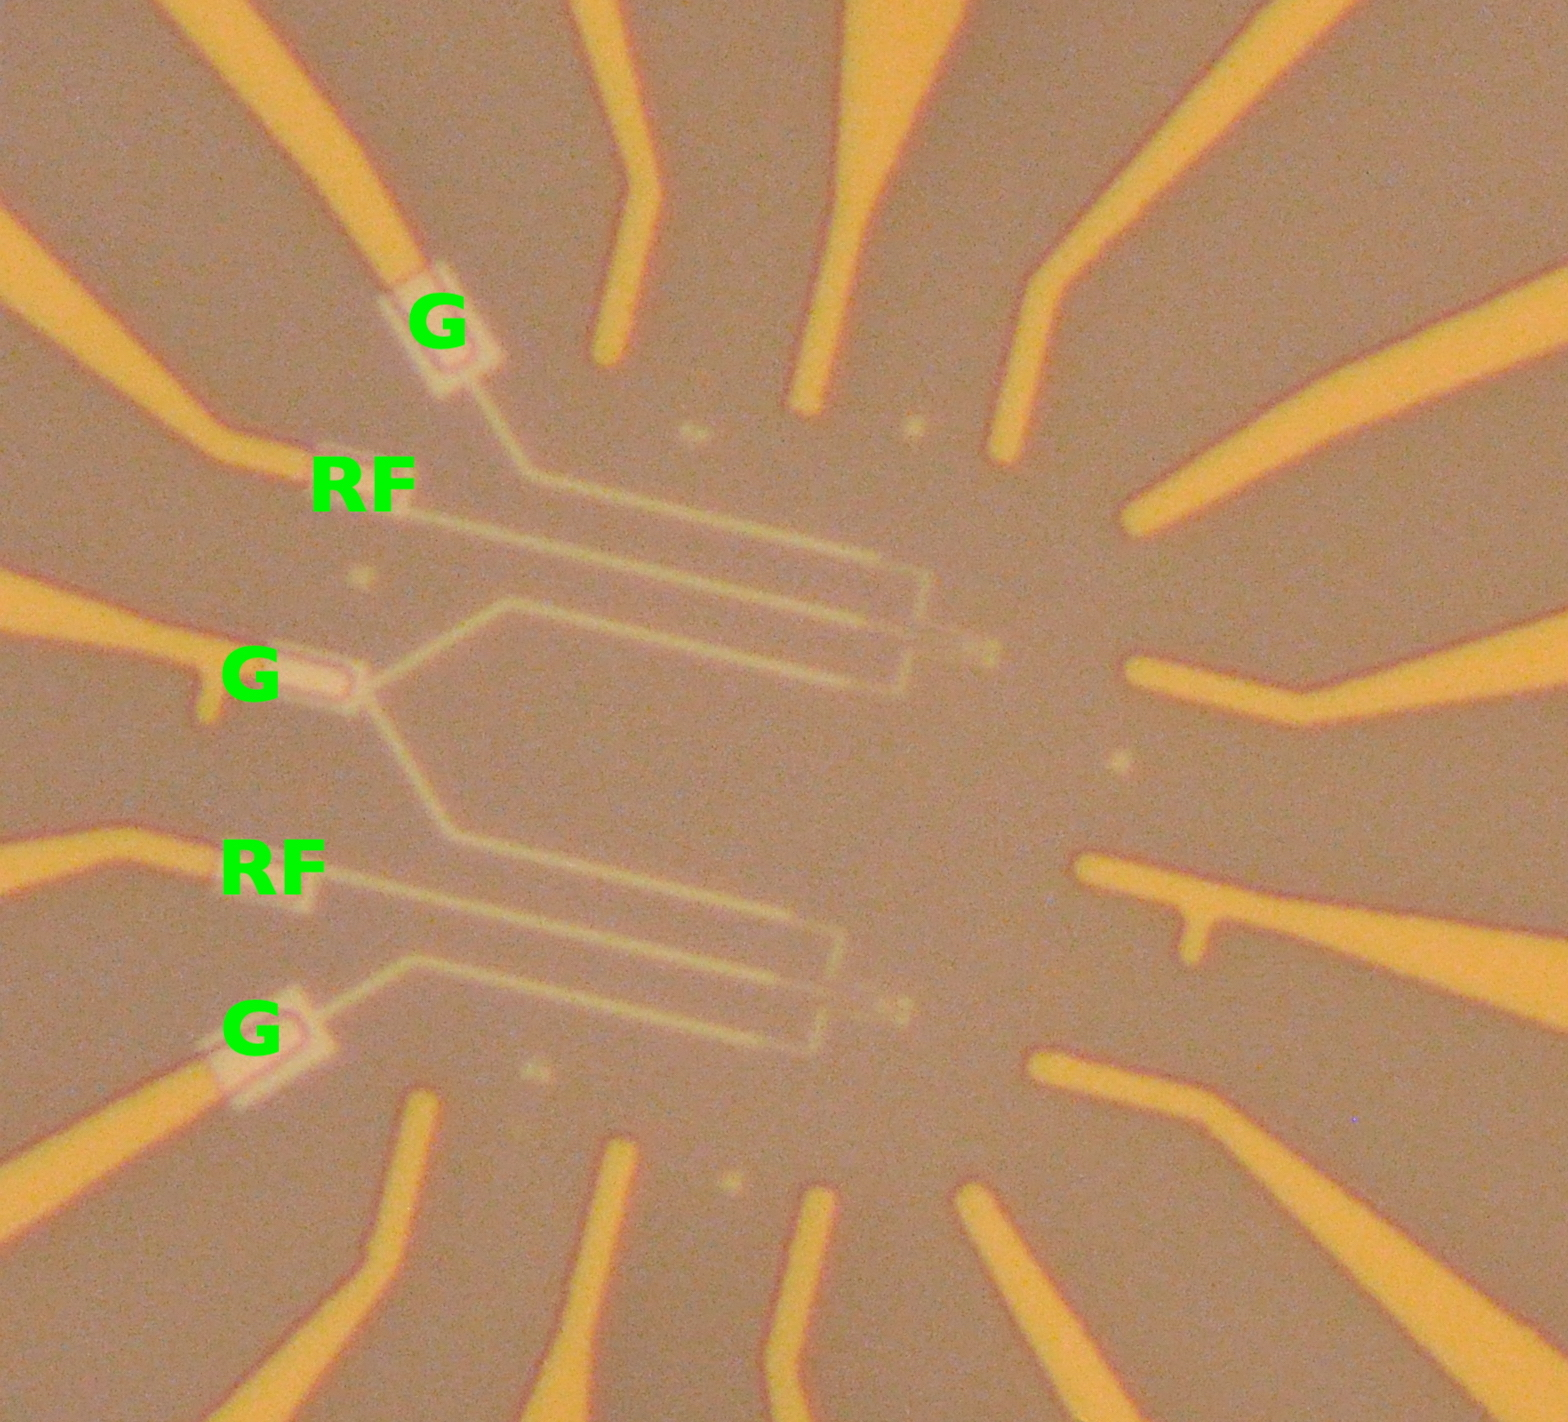
\includegraphics[height=2cm]{F}
\end{figure}

\begin{itemize}
\item The RF bias is on the RHS of the PCB;
\item Numeration of  contacts on the PCB begin below  the RF line and
  goes clockwise;
\item Position 2 is on top, Position 1 is on bottom (remember to flip
  the chips);
\item \red{Attach with small drop of resin \textbf{so that chip 1 and
      chip 2 are exposed to contacts 1,2,3,4};}
\item Remove with scalpel and wash chips in acetone.
\end{itemize}

 \begin{figure}[h]
   \centering%
   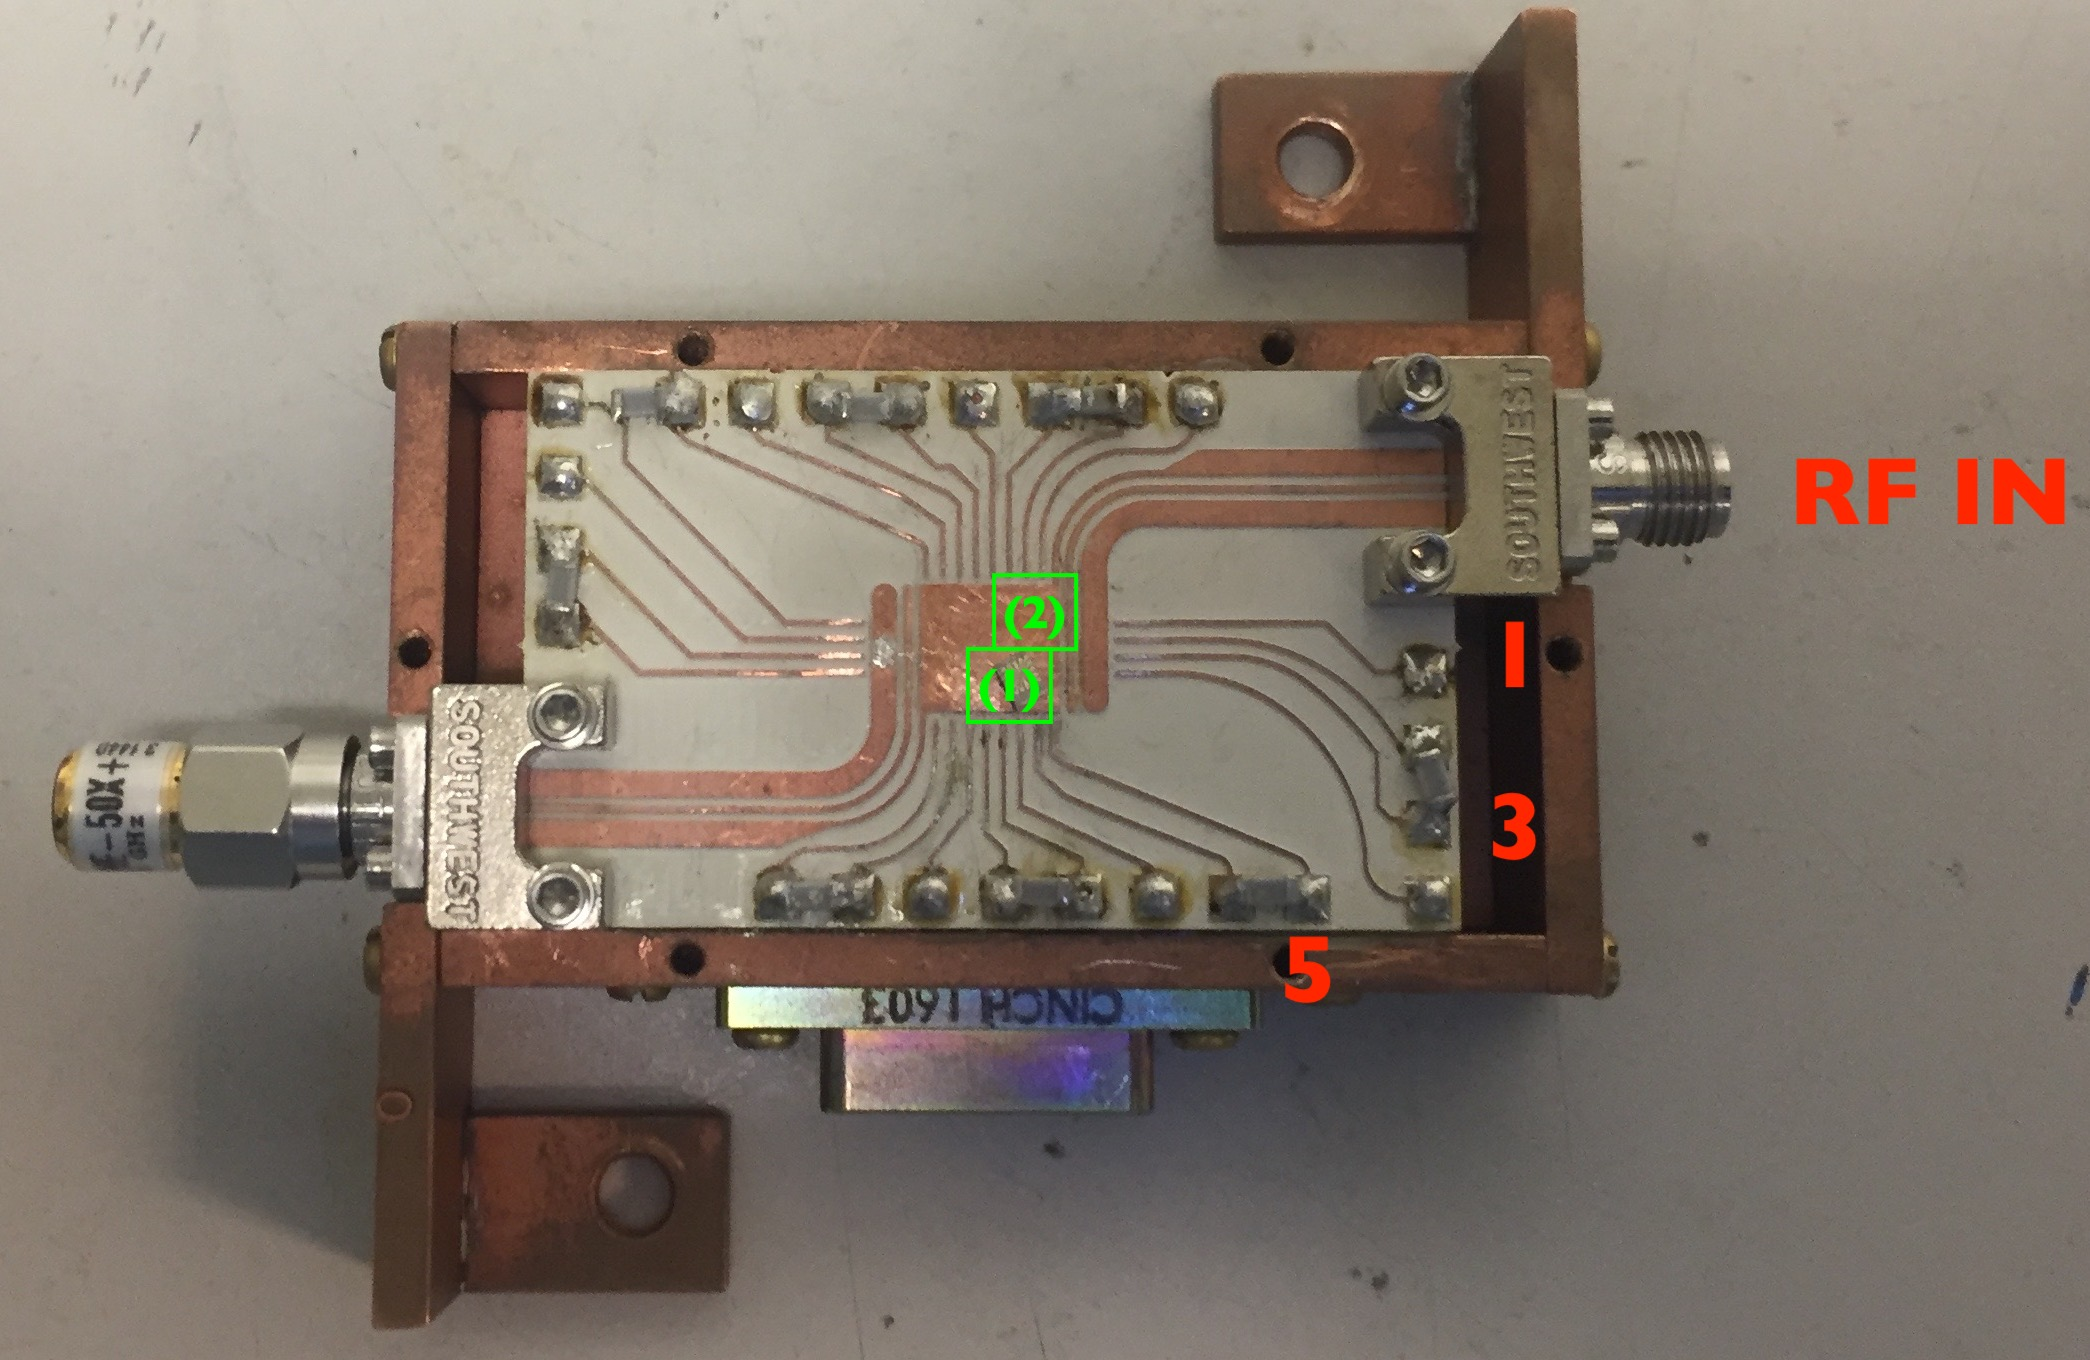
\includegraphics[height=5cm]{pcb1}%
   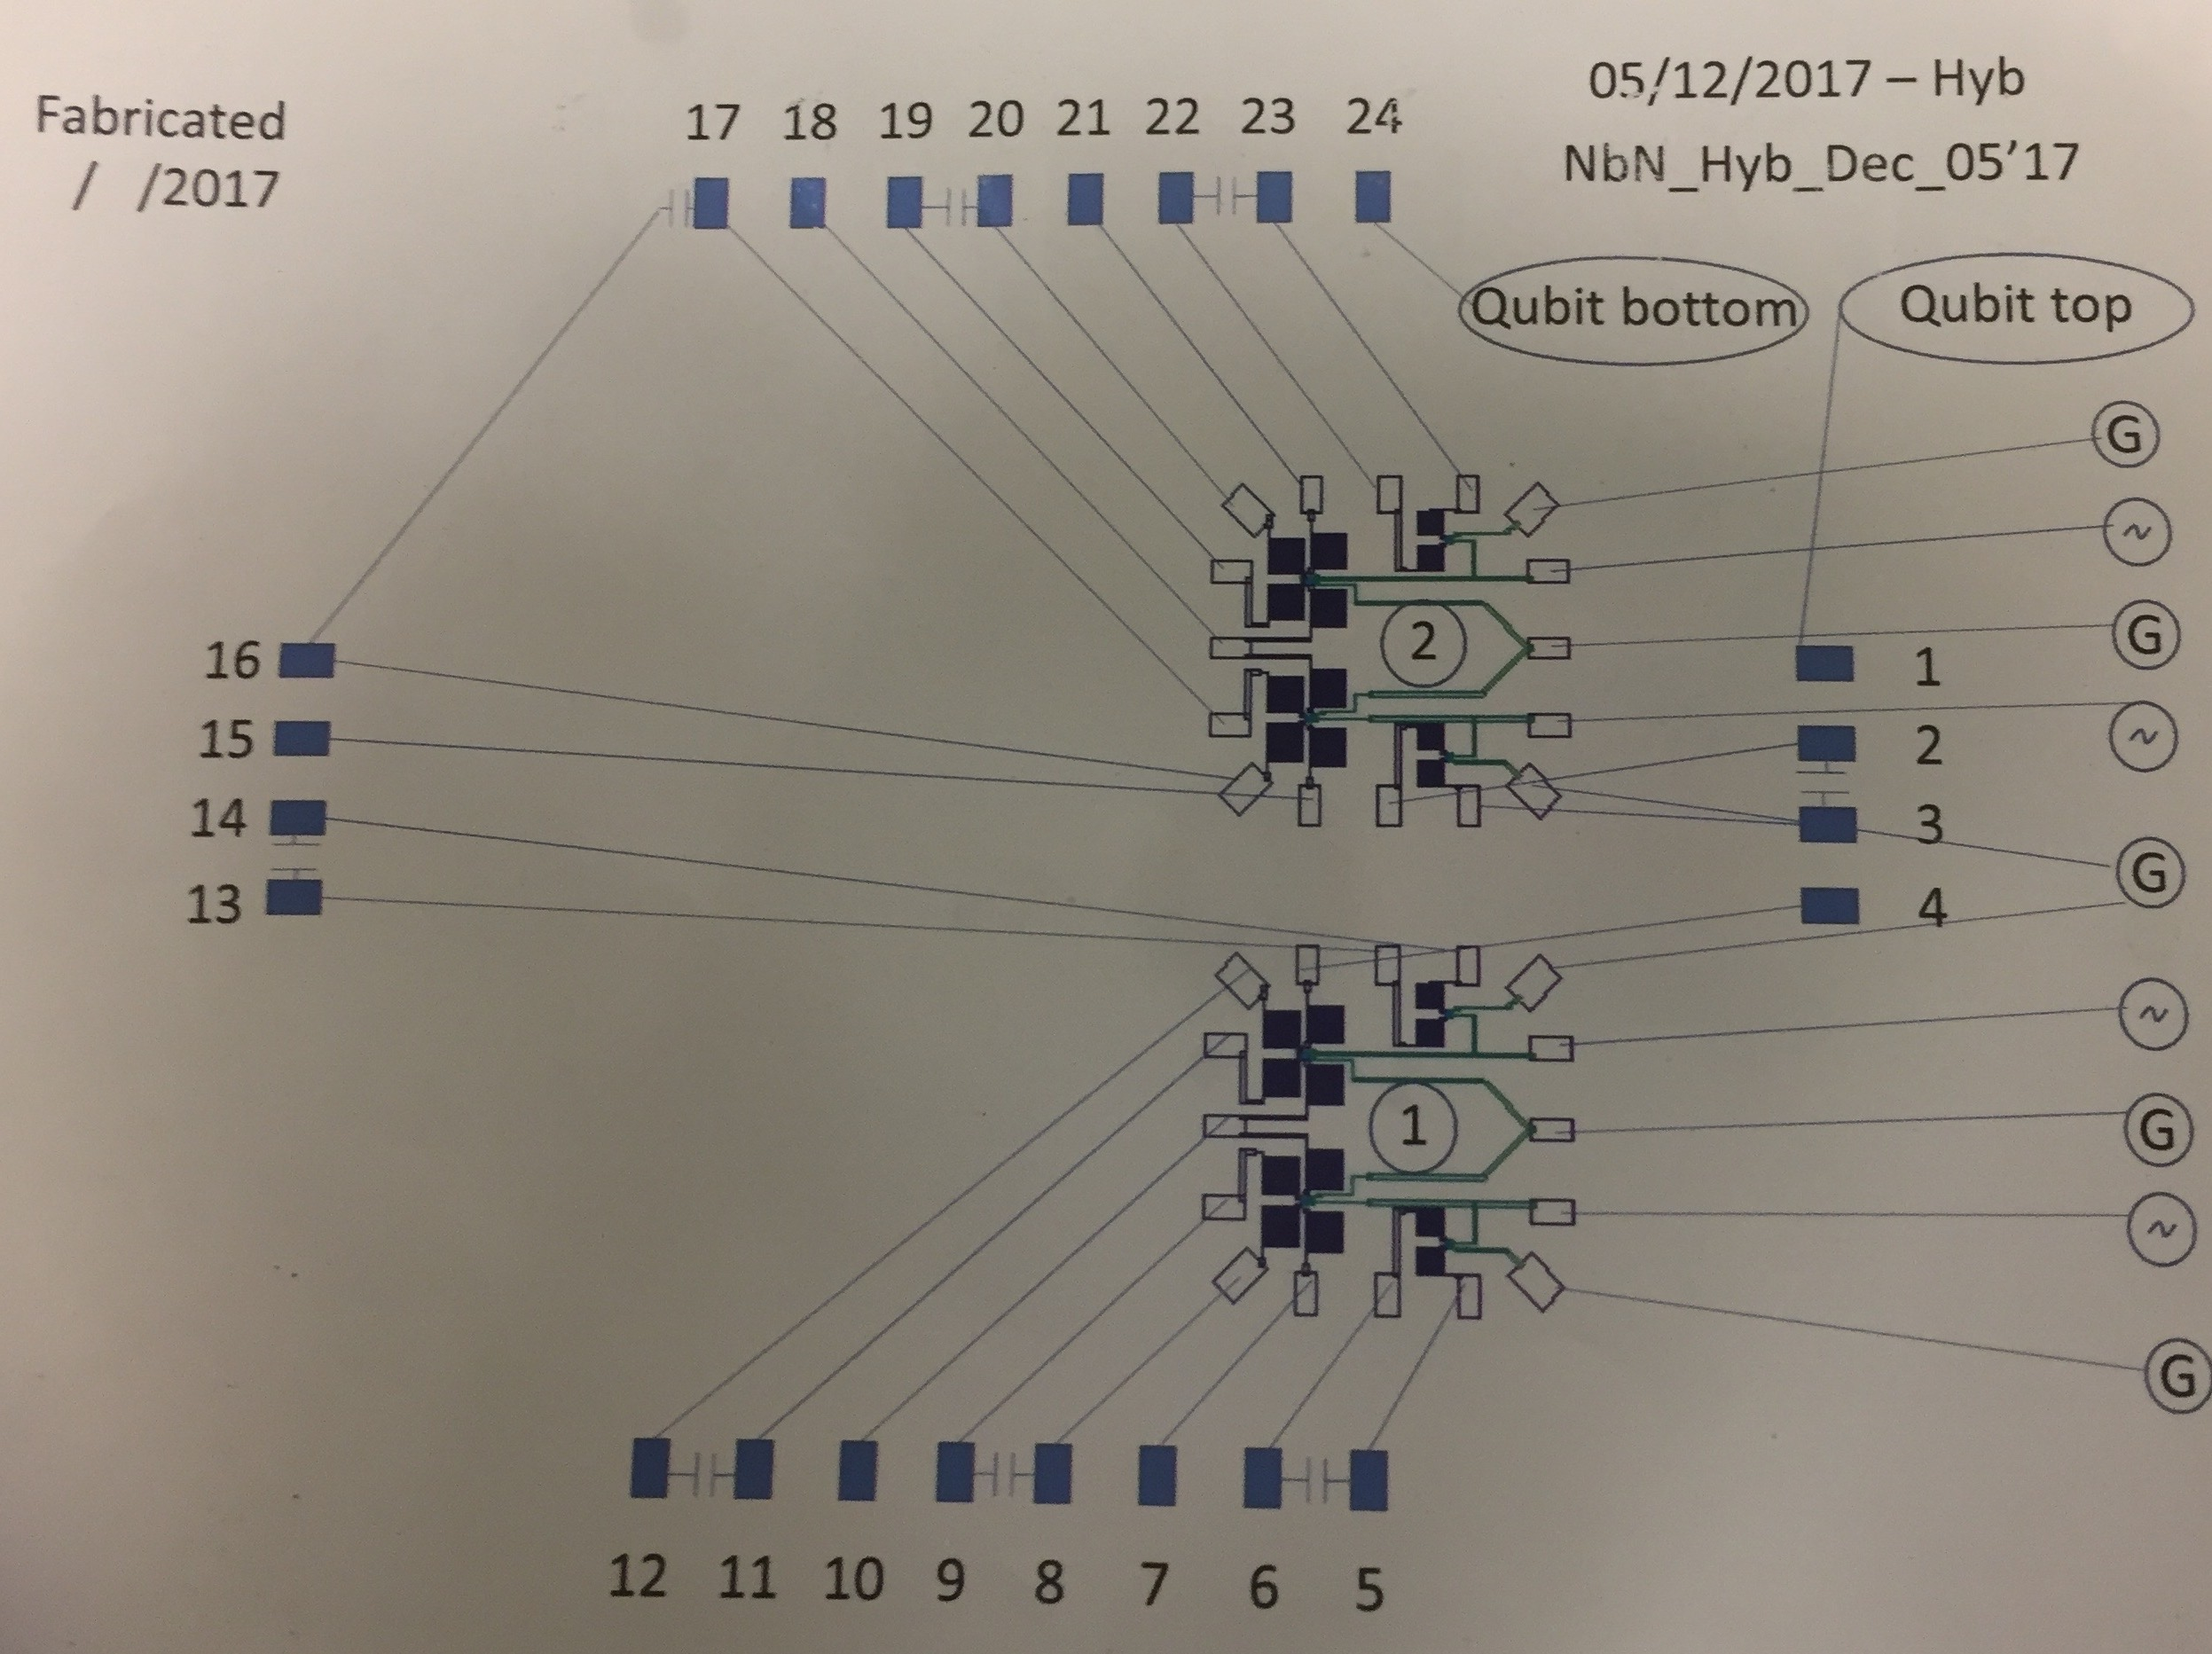
\includegraphics[height=5cm]{pcb2}%
 \end{figure}
 \newpage
